\chapter{Event Reconstruction and Section}\label{chapt:event_selection}

The reconstruction procedure is interpreting the outcoming detector data as a set of physical objects.

In general, for this analysis each object of the $t\bar{t}$ dileptonic final state was reconstructed using the \textit{Particle Flow} (PF)
algorithm \cite{Beaudette:2014cea}. It is an iterative process which reconstructs the particles and jets exploiting the information from all parts
of the detector. After an object is reconstructed in one iteration, all the detector signals assigned to it are blinded for the further iterations.

The reconstruction with the PF algorithm following \cite{Beaudette:2014cea} starts with muons as they are the most unambiguous particles to identify.
After blinding the muon signals in the detector, the charged hadrons are reconstructed. The next step is the electron reconstruction and afterwards
all the remaining signals are assigned to the neutral hadrons and photons. After all particles are reconstructed and identified, the missing transverse
energy ($E_{T}^{miss}$) is constructed out of them. A complete overview of the PF algorithm can be found in \cite{CMS-PAS-PFT-09-001}. 

Different algorithms and methods are used to reconstruct different objects and some of them (relevant for this analysis -- leptons, jets and missing transverse
energy, responsible for neutrinos) are discussed in this chapter. Finally the selection which aims to suppress the $t\bar{t}$ like events
with the similar final state signature and increase the event quality is presented. The selection is based on the CMS Top-Quark-Physics-Analysis group recommendations \cite{TopPAGreco}.

%%%%%%%%%%%%%%%%%%%%%%%%%%%%%%%%%%%%%%%%%%%%%%%
\section{Track and Vertex Reconstruction}

Tracks\footnote{A \textit{track} is a set of information about the charged particles trajectory curve and momentum.} and vertecies\footnote{A 
\textit{vertex} is an estimate of a point in space where the particles arise from. It can be either related to the 
collision point or to the place  where some secondary interaction happened.} are the essential objects used for all the particles reconstruction. 
However they are not the primer detector output and they have to be reconstructed.

\subsection{Track Reconstruction}\label{ssec:trkReco}

The track reconstruction has to take place using the information from the inner tracking detectors. The neighboring pixels and strips which
produce signals are grouped to clusters. A position of a cluster defines a hit which is an estimate of the point where a particle crossed the
detector material. A particle trajectory can be tracked if fitting the corresponding consequence of hits. A curvature 
of the trajectory with the known magnetic field gives a momentum estimate of a particle.

The track reconstruction procedure consists of four main steps as following \cite{Chatrchyan:2014fea}:

\begin{itemize}
 \item \textbf{Seed generation}: all the possible combinations of three points (3 hits in the first layers of pixel tracker or beam spot center\footnote
 {A primary interaction region or a \textit{beam spot} is defined as an average value over all the events and is defined as a most luminous point.} and
 two hits from the first tracker layers) are fitted with a helical trajectory assuming the quasi-uniform magnetic field. Every fitted object is required
 to have some minimum $p_{T}$, maximum beam spot impact parameter\footnote{An \textit{impact parameter} $d_{xy}$ of the track is a minimum
 distance of the track to certain vertex or beam spot in the transverse $x-y$ plane.} and correct charge distribution requirements to be accepted
 as an initial track candidate or seed.
 %
 \item \textbf{Track finding}: extrapolates the seeding candidates along the expected flight paths to the consecutive tracking detector layers searching 
 for the new hits and reestimating the track parameters respectively. On each consecutive layer all the hits from the 3 sigma region around the seed trajectory
 are taken and fitted with a Kalman filter\cite{Fruhwirth:1987fm}. The best $\chi^{2}$ hit is taken and the trajectory
 continues extrapolation to the next layer until the end of tracker is reached. In case no hit is found on some layer a ghost hit is assumed. The track is not
 accepted if it contains more then one ghost hit.
 %
 \item \textbf{Track fitting}: after finding the hits in all the tracker layers with the track finding, a track candidate is refitted using the Kalman filter. 
 This procedure is performed releasing the constrains set on the seeding stage.
 %
 \item \textbf{Track selection}: reduces the rate of fake tracks\footnote{A \textit{fake track} is a track produced by the fit but is actually there was
 no real charged particle which produced this track.} by setting physical and quality constrains on the object produced at the previous step. The requirements
 are based on a good $\chi^{2}$ and reasonable impact parameter value to the beam spot.
\end{itemize}

The tracking procedure is repeated in several iterations.
%Each iteration differs in the set of $p_{T}$ and beam spot impact parameter
%requirements for the seed tracks generation\cite{Chatrchyan:2014fea}. 
The first iteration has the hardest requirements - high $p_{T}$ of the tracks
and a good connection to the beam spot center (such objects are usually easier to reconstruct). After reconstructing the tracks in the first iteration,
their hits are removed and the second iteration starts with a bit softer requirements on the seed tracks. In total, six iterations are performed.
% 
% For the HLT (see sec.\ref{sec:trig}) track reconstruction the information from pixel tracker only is used, repeating the seed generation procedure\cite{Chatrchyan:2014fea}.
% This procedure is fast enough for the trigger performance. However the tracks produced this way have a higher probability to be fake and have worse resolution, they
% are not used as the track candidates, but rather for the vertex reconstruction at the trigger level. To define track candidates a simplistic procedure
% involving pixel and strip detector information is performed on the HLT\cite{Chatrchyan:2014fea}.

\subsection{Primary Vertex Reconstruction}\label{ssec:vtxReco}

The primary vertex reconstruction aims to measure the location of all proton-proton collision points in the event (see Figure \ref{fig:HugePU}). The reconstruction procedure has three
phases described as follows\cite{Chatrchyan:2014fea}:

\begin{figure}[t]
  \centering
  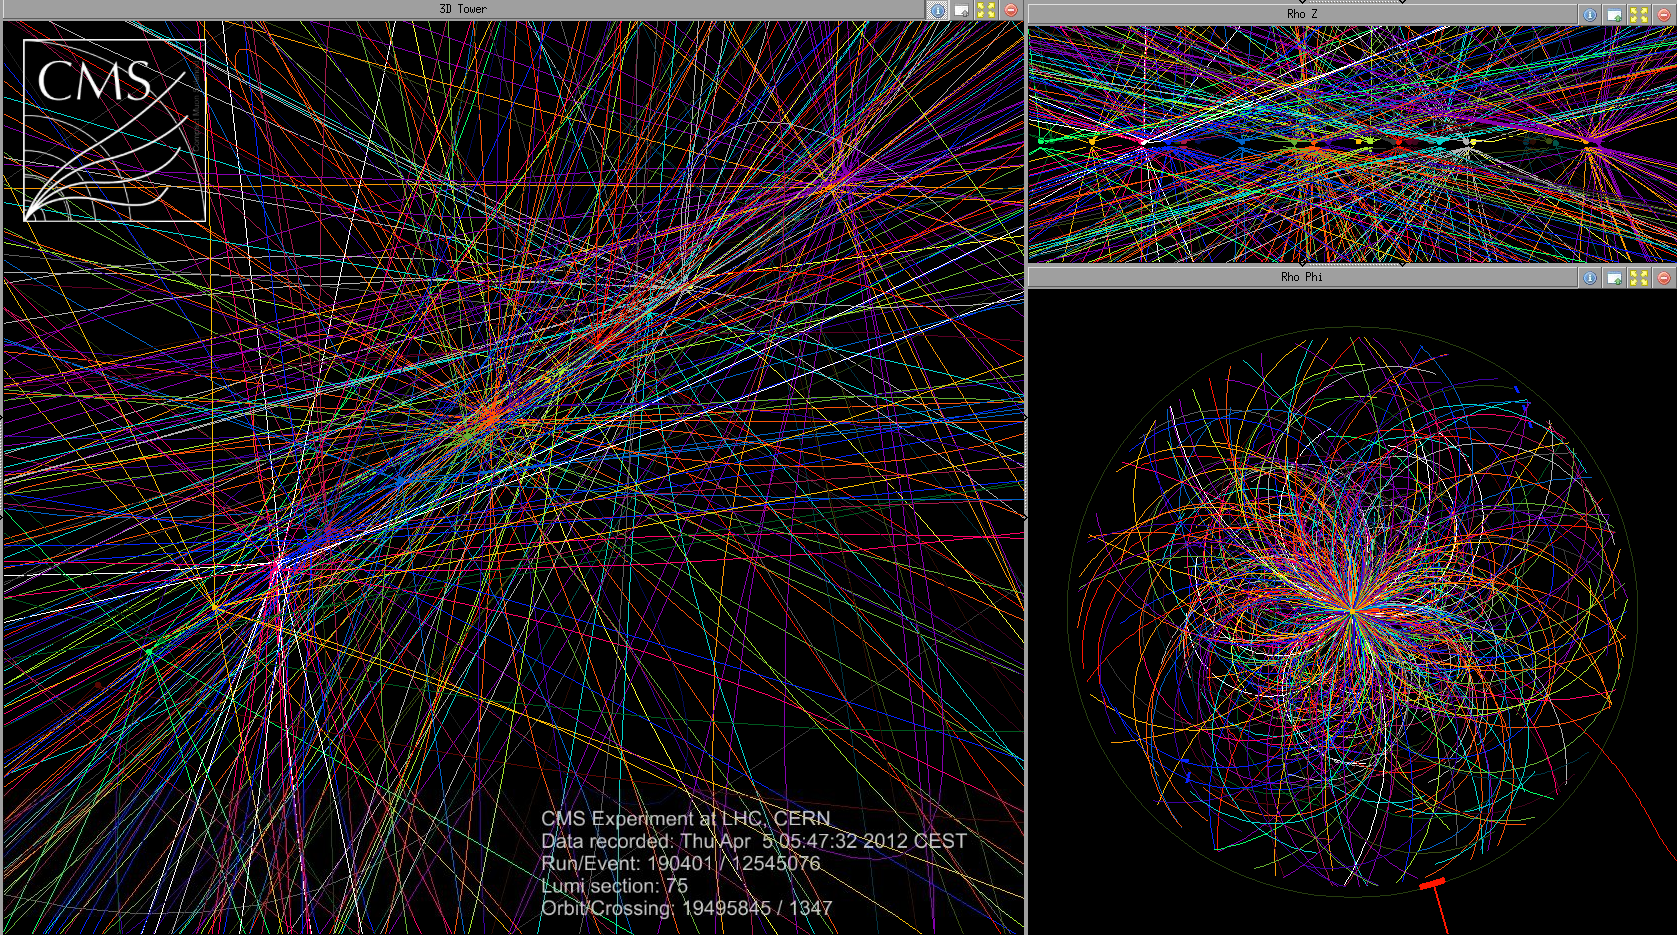
\includegraphics[width=1.0\textwidth]{04_event_reconstruction/plots/url.png}
  \caption{Magnified view of the event showing 29 distinct vertices reconstructed corresponding to 29 distinct collisions within a single crossing of the LHC beam.}
  \label{fig:HugePU}
\end{figure}
\begin{itemize}

 \item \textbf{Track selection}: the tracks for the primary vertex reconstruction are chosen with certain requirements such as to be consistent with being produced 
 in the primary interaction region (the significance of the beam spot impact parameter -- it's value over it's uncertainty -- has to be maximum 5), having at least two pixel 
 layers and at least five pixel and strip layers associated with the track and having the $\chi^{2}$ per degree of freedom of the track fit not higher then 20.
 %
 \item \textbf{Track clustering}: the main task of the clustering algorithm is to separate the groups of tracks emerging from different primary vertecies, not splitting 
 the tracks from one vertex to two, but also not merging the tracks from different vertecies to one. The tracks are clustered according 
 to their $z$-coordinate at the point of closest approach to the beam spot center. 
 \\
 The algorithm used for clustering for the CMS 2012 data is the \textit{deterministic annealing} described in detail in\cite{rose_ieee1998}. The system with many tracks has many degrees
 of freedom and finding the primary vertex regions according to the coordinates of the closes approach to the beam spot center is treated analogically to the problem of a physical 
 system approaching a state of minimal energy through a series of gradual temperature reductions.
 %
 \item \textbf{Fitting the position of the vertex}: each clustered group of tracks forms a vertex candidate. Only the candidates with at least two tracks are taken and are fitted
 using the \textit{adaptive vertex fitter}\cite{Frühwirth:1027031}. The output of the fit is the vertex position, it's uncertainty and $\chi^{2}$. The determination of the probability
 of each track to arise from the reconstructed vertex is performed.
\end{itemize}

The information on all primary vertecies in the event is useful not only for other objects reconstruction but also for separating the signal vertex (with hard interaction) 
from the others with no useful physics information.

%%%%%%%%%%%%%%%%%%%%%%%%%%%%%%%%%%%%%%%%%%%%%%%
%%%%%%%%%%%%%%%%%%%%%%%%%%%%%%%%%%%%%%%%%%%%%%%
%%%%%%%%%%%%%%%%%%%%%%%%%%%%%%%%%%%%%%%%%%%%%%%
\section{Objects Reconstruction}

The reconstruction of the muons, electrons, jets and missing transverse energy ($t\bar{t}$ dileptonic final state objects)
is presented in this section.

%%%%%%%%%%%%%%%%%%%%%%%%%%%%%%%%%%%%%%%%%%%%%%%
\subsection{Muon Reconstruction}

As it was discussed in section \ref{sec:CMS}, the CMS experiment has a well established setup for the muon reconstruction.
Muons are the only particles expected to appear in the muon sub-detector system, thus their identification is unambiguous.
Figure \ref{fig:PFmuons} shows a muon path in the detector compared to the other particles.
One can get three types of muons out of the reconstruction:

\begin{figure}[t]
  \centering
  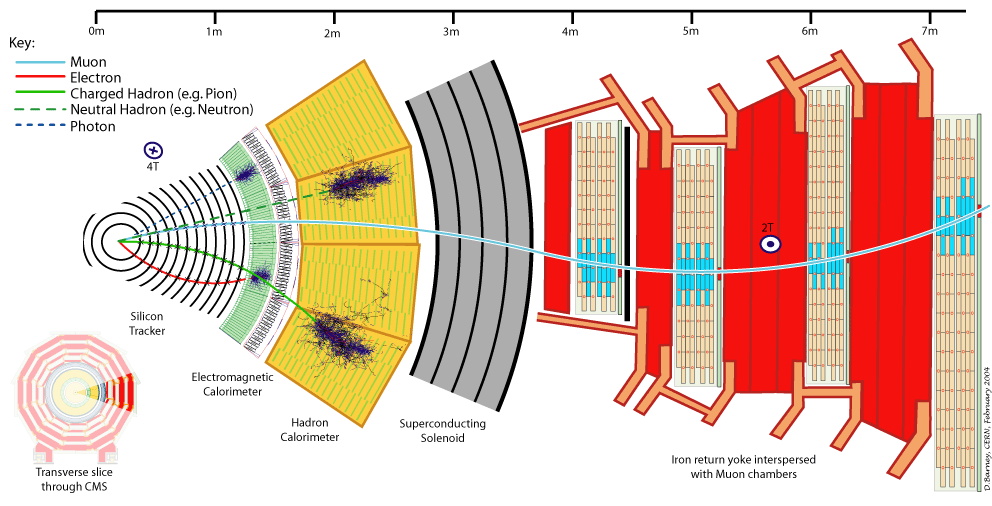
\includegraphics[width=1.0\textwidth]{04_event_reconstruction/plots/CMS_Slice.png}
  \caption{Track reconstruction using different sub-detector information in combination in Particle Flow algorithm. An actual
  muon track is shown with a curved blue line, an electron track is red and a charged hadron is solid green.}
  \label{fig:PFmuons}
\end{figure}

\begin{itemize}
 \item \textbf{Standalone}: muon tracks are reconstructed using the information from the muon system only. The track reconstruction
 algorithm \cite{TWiki:GlobalMuon} is similar to the one used in the tracking system. Here the analogue to the
 tracker cluster is a segment in any part of the muon detector.
% \\
%  The first stage, \textit{seed generation}, needs 3 parameters to fit a muon seed (as in sec.\ref{ssec:trkReco}). These can be either a beam spot position, segment position and segment
%  bending angle with respect to the vertex direction or two segments from MB3 and MB4 (see figure \ref{fig:muond} in sec.\ref{ssec:muonDet}) and the difference
%  between their bending angles. Also, the algorithm allows to take two segments from the first muon stations, MB1 and MB2, beam spot position and their
%  bending angles, determine a seed for each of them and take an average. In the CSC region (see sec.\ref{ssec:muonDet}) the two segments from first and second
%  or first and third stations are taken with either the difference between their $\phi$ coordinate or the direction of the higher quality segment as a bending parameter.
%  The muon seed generation algorithm is used for the HLT muon track definition.
%  \\
%  The further procedure is to extrapolate the tracks to the other layers of the muon system (it is flexible enough to prolong the tracks from the outermost layers inside or
%  from the innermost layers outside, depending on how the seed was created). The track propagation is performed using the Kalman filter. Each time a new point of the 
%  track is found, the track is refitted (taking into account the effects from the multiple interaction with matter). In case on any step the $\chi^2$ per degree of freedom 
%  of the fit turns out to be higher then 20, this track is rejected. 
 
 \item \textbf{Tracker}: the tracks, reconstructed in the tracking detector only as described in sec. \ref{ssec:trkReco}, 
 are assigned as muons in case they match at least one hit in the muon sub-detector \cite{TWiki:GlobalMuon}.
 
 \item \textbf{Global}: the muons are reconstructed using 
 the combined fit of tracks from the muon system and from the inner tracker. Here the standalone and tracker muons are fitted together. The details are given
 in \cite{TWiki:GlobalMuon}.
\end{itemize}

%%%%%%%%%%%%%%%%%%%%%%%%%%%%%%%%%%%%%%%%%%%%%%%
\subsection{Electrons reconstruction}\label{ssec:ElRec}

The electrons are reconstructed by coming the tracks from tracker with the clusters from ECAL. The electron seeds
are created making use of two complementary algorithms as following \cite{CMS-PAS-EGM-10-004}: \textit{tracker driven seeding}, 
which is performed for the tracks with the $p_{T} < 5$ GeV matching the tracks from the tracker to the ECAL superclusters\footnote
{A \textit{supercluster} is a group of one or more associated clusters of energy deposits in the ECAL. The transverse energy $E_{T}$
of the supercluster has to be not lower then 4 GeV.}, and \textit{ECAL driven seeding}, performed for the tracks with $p_{T} \geq 5$ GeV
fitting the ECAL superclusters to the tracker tracks. All the seeds are fitted with the Gaussian Sum Fitter \cite{GSF_Electron_Reconstruction_CMS}
using the hypothesis that each track is an electron and assuming the dedicated energy losses.

On the next reconstruction step the fitted seeding tracks are preselected. The tracker seeds are preselected by the multivariate analysis 
(MVA) as described in \cite{CMS:2010byl}. For the ECAL seeds the restrictions on the GSM matching in $\eta$ and $\phi$ are applied \cite{Baffioni:2006cd}.

The collection of the tracks formed after the preselection is assigned to electrons.

%%%%%%%%%%%%%%%%%%%%%%%%%%%%%%%%%%%%%%%%%%%%%%%
\subsection{Jet Reconstruction}

A quark or a gluon as a colorful object can't exist singly due to the confinement property (see sec. \ref{sec:quark}).
A quark thus starts to hadronize and form a group of particles (primarily hadrons only) flowing in one direction. These are the jets. Special algorithms are developed
to find and reconstruct jets.

\subsubsection{Jet Finder Algorithms}

The idea which lies behind any algorithm of a jet finding and reconstruction is the merging of the objects which are measured near by in the detector.
Generally a jet can be reconstructed using two strategies \cite{Salam:2007xv}:

\begin{itemize}
 \item \textit{Sequential clustering}: the particles are sequentially recombined until the closest (regarding the actual distance between measured
 objects) combination is found.
 %
 \item \textit{Cone algorithms}: a jet is defined as a cone around some direction of dominant energy flow. Each or some of the particles are tried 
 in a role of the dominant direction seed. The next step was to define a trial cone around the seed and accept all the particles which enter this cone.
 The sum of the four-momenta of all objects inside the jet candidate area is calculated. This jet candidate is assumed to be a new seed. This iterative process continues
 until the stable seed is found.
\end{itemize}

Although the cone algorithms are fast and simplistic they are not collinear and infrared safe by default.

The sequential clustering algorithms are both infrared and collinear safe. They don't rely on a stable cone. The procedure of constructing
a jet starts with defining two distances -- $d_{ij}$ (the distance between two objects, particles or pseudojets, $i$ and $j$ in the detector) and $d_{iB}$ (the distance between the object $i$
and the beam spot). These two distances are compared:

\begin{itemize}
 \item [--] $d_{ij} < d_{iB}$: the objects $i$ and $j$ are combined together to a pseudojet which enters the algorithm again as a single object;
 \item [--] $d_{ij} > d_{iB}$: the object $i$ is taken as a final jet.
\end{itemize}

The different sequential clustering algorithms differ at the level of the distance definition. In general the distances are defined as follows \cite{Cacciari:2008gp}:

\begin{align}
 d_{ij} & = min(k_{Ti}^{2p}, k_{Tj}^{2p}) \frac{\Delta_{ij}^{2}}{R^{2}},\label{eq:ktDist} \\
 d_{iB} & = k_{Ti}^{2p}, \\
 \Delta_{ij}^{2} & = (y_{i} - y_{j})^{2} + (\phi_{i} - \phi_{j})^{2}.
\end{align}

Here the $k_{Ti}$, $y_{i}$ and $\phi_i$ are the transverse momentum, rapidity and azimuth angle of an object $i$. The $R$ is a cone radius which tells 
how large the jet can be. A $p$ is the parameter which varies the power of the energetic term in comparison to the geometrical scale $\Delta_{ij}$.
There are three different sequential clustering algorithms depending on the $p$ value:

\begin{itemize}
 \item $p = 1$ defines the $k_{T}$ algorithm, where the energetic and spatial term are of the same power;
 \item $p = 0$ defines the Cambridge/Aachen algorithm, where the energetic term in eq.\ref{eq:ktDist} is removed thus the spatial part only plays role;
 \item $p = -1$ defines the anti-$k_{T}$ algorithm.
\end{itemize}

The jets for this analyses were constructed making use of the anti-$k_{T}$ sequential clustering algorithm. 

\subsubsection{Jet Energy Calibration}\label{ssec:JCal}

The reconstructed jet energy should be corrected for the non-linear and non-uniform responses of the calorimeter. For this a factorized jet calibration
method is used \cite{2011JInst...611002C}. Calibration is performed sequentially in several steps displayed:

\begin{itemize}
 \item \textit{Offset correction} removes extra energy due to electronics noise and pile-up. Applied on the real and simulated reconstructed data.
 %
 \item \textit{Monte Carlo calibration} corrects the energy of the reconstructed jets such that it is equal to the average energy of the generated 
 particle jets. This correction is performed in bins of the jets $p_{T}$ and $\eta$. Applied on the simulated reconstructed data.
 %
 \item \textit{Relative jet energy correction} ensures a flat response depending on $\eta$. Applied on the simulated reconstructed data
 %
 \item \textit{Absolute jet energy correction} balances the $p_{T}$ response to be linear. It is calibrated on the well reconstructed $Z^{0}$
\end{itemize}


First calibration step deals with the additional energy in the jet which does not occur from a hard process but rather from the detector noise or pile up. 
Obviously this correction produces the factor always smaller then 1 thus the jet energy reduces on this step. Further correction steps aim to make the jet response
flat as a function of $|\eta|$ and $p_{T}$. The correction on the geometrical position dependence corrects all the energies as if they were measured 
in the most efficient barrel region using the dijet data events. The $p_{T}$ dependence correction makes use of the Drell-Yan events to exploit a good
lepton energy and momentum resolutions. Finally the residual corrections are applied on data to correct for some minor disagreement with the simulation.

In general all the corrections factor in the kinematic region of interest for this analysis are smaller then $5\%$.

\subsubsection{b-Jets identification}\label{ssec:bTag}

The task of the $b$-jet identification is to distinguish a $b$-quark jet from the light flavour-, $c$- and gluon-jets. In particular,
a long life time of the B hadrons (in the order of $10^{-12}$ s) which allows it to travel far enough from the primary interaction point (about 500 $\mu$m) before the decay
may be exploited. The point in space, which corresponds to the place of $B$-hadron decay can be reconstructed in the pixel tracking detector as a \textit{secondary vertex}. 
An important parameter which can be used to identify the jet origin is the impact parameter of the tracks arising from the secondary vertex (see Figure \ref{fig:SV}).

\begin{figure}[t]
  \centering
  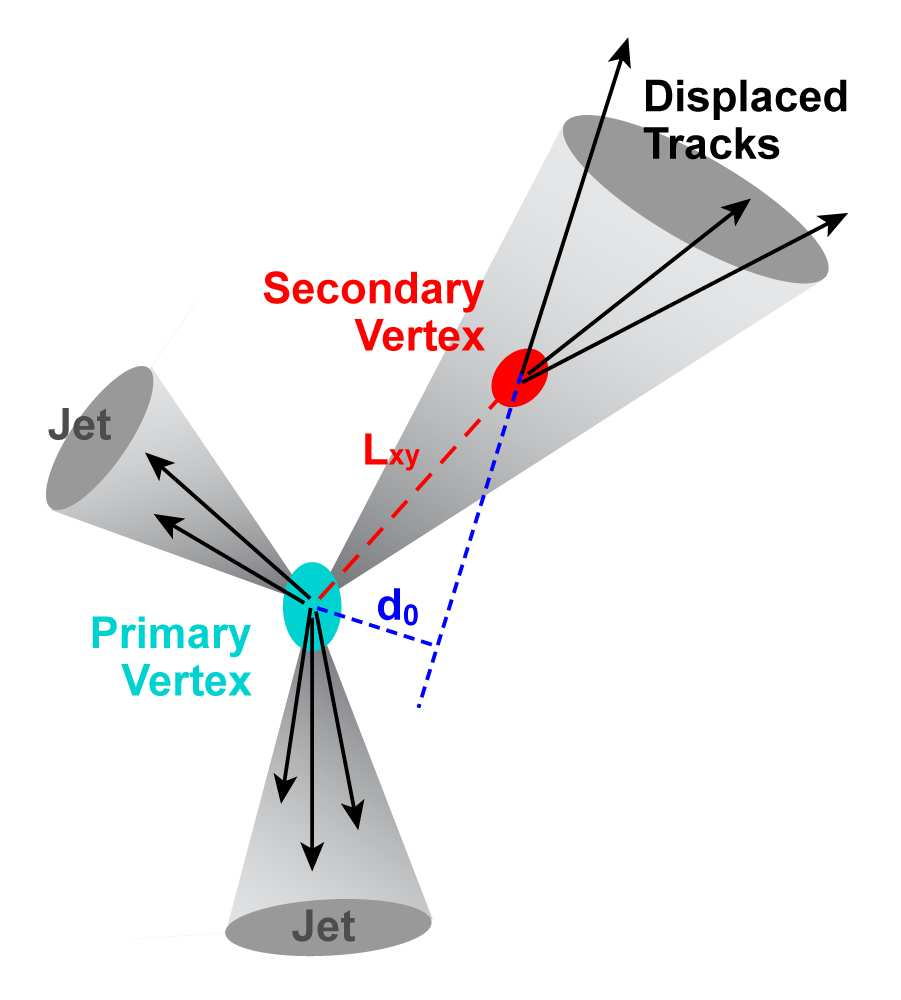
\includegraphics[width=0.5\textwidth]{04_event_reconstruction/plots/btagging_cartoon.png}
  \caption{A sketch of the event with a reconstructed secondary vertex. A light blue circle is the primary vertex and a red circle is the secondary vertex. The impact 
  parameter of a track is marked with a blue dashed line and a symbol $d_{0}$.}
  \label{fig:SV}
\end{figure}

The algorithm used for this analysis is called \textit{Combined Secondary Vertex} (CSV) \cite{CMS-PAS-BTV-13-001}. It defines a likelihood-based discriminator which uses 
the lifetime information to distinguish $b$-jets, $c$-jets and light jets.

The minimum thresholds for the algorithm are defined as three \textit{working points}, loose (L), medium (M) and tight (T), as following \cite{CMS-PAS-BTV-13-001}:

\begin{itemize}
 \item [--] CSVL sets the threshold on the actual discriminator value as $\geq 0.244$, which has an efficiency $\sim 80\%$ and a misidentification probability of
 light hadron jets close to $10\%$;
 %
 \item [--] CSVM sets a harsher threshold on the discriminator value of $\geq 0.679$, which lowers the misidentification probability to $\sim 1\%$, but also
 reduces the statistics down to 65$\%$;
 %
 \item [--] CSVT has the hardest threshold on the discriminator value of $\geq 0.898$. This lowers the misidentification probability by other factor of 10 ($0.1\%$)
 and reduces the efficiency down to 50$\%$;
\end{itemize}

In general the efficiency of the CSV algorithm was estimated in data and simulated QCD events \cite{CMS-PAS-BTV-13-001}. The resulting curve is presenter on the figure \ref{fig:CSVeff}.

\begin{figure}[t]
  \centering
  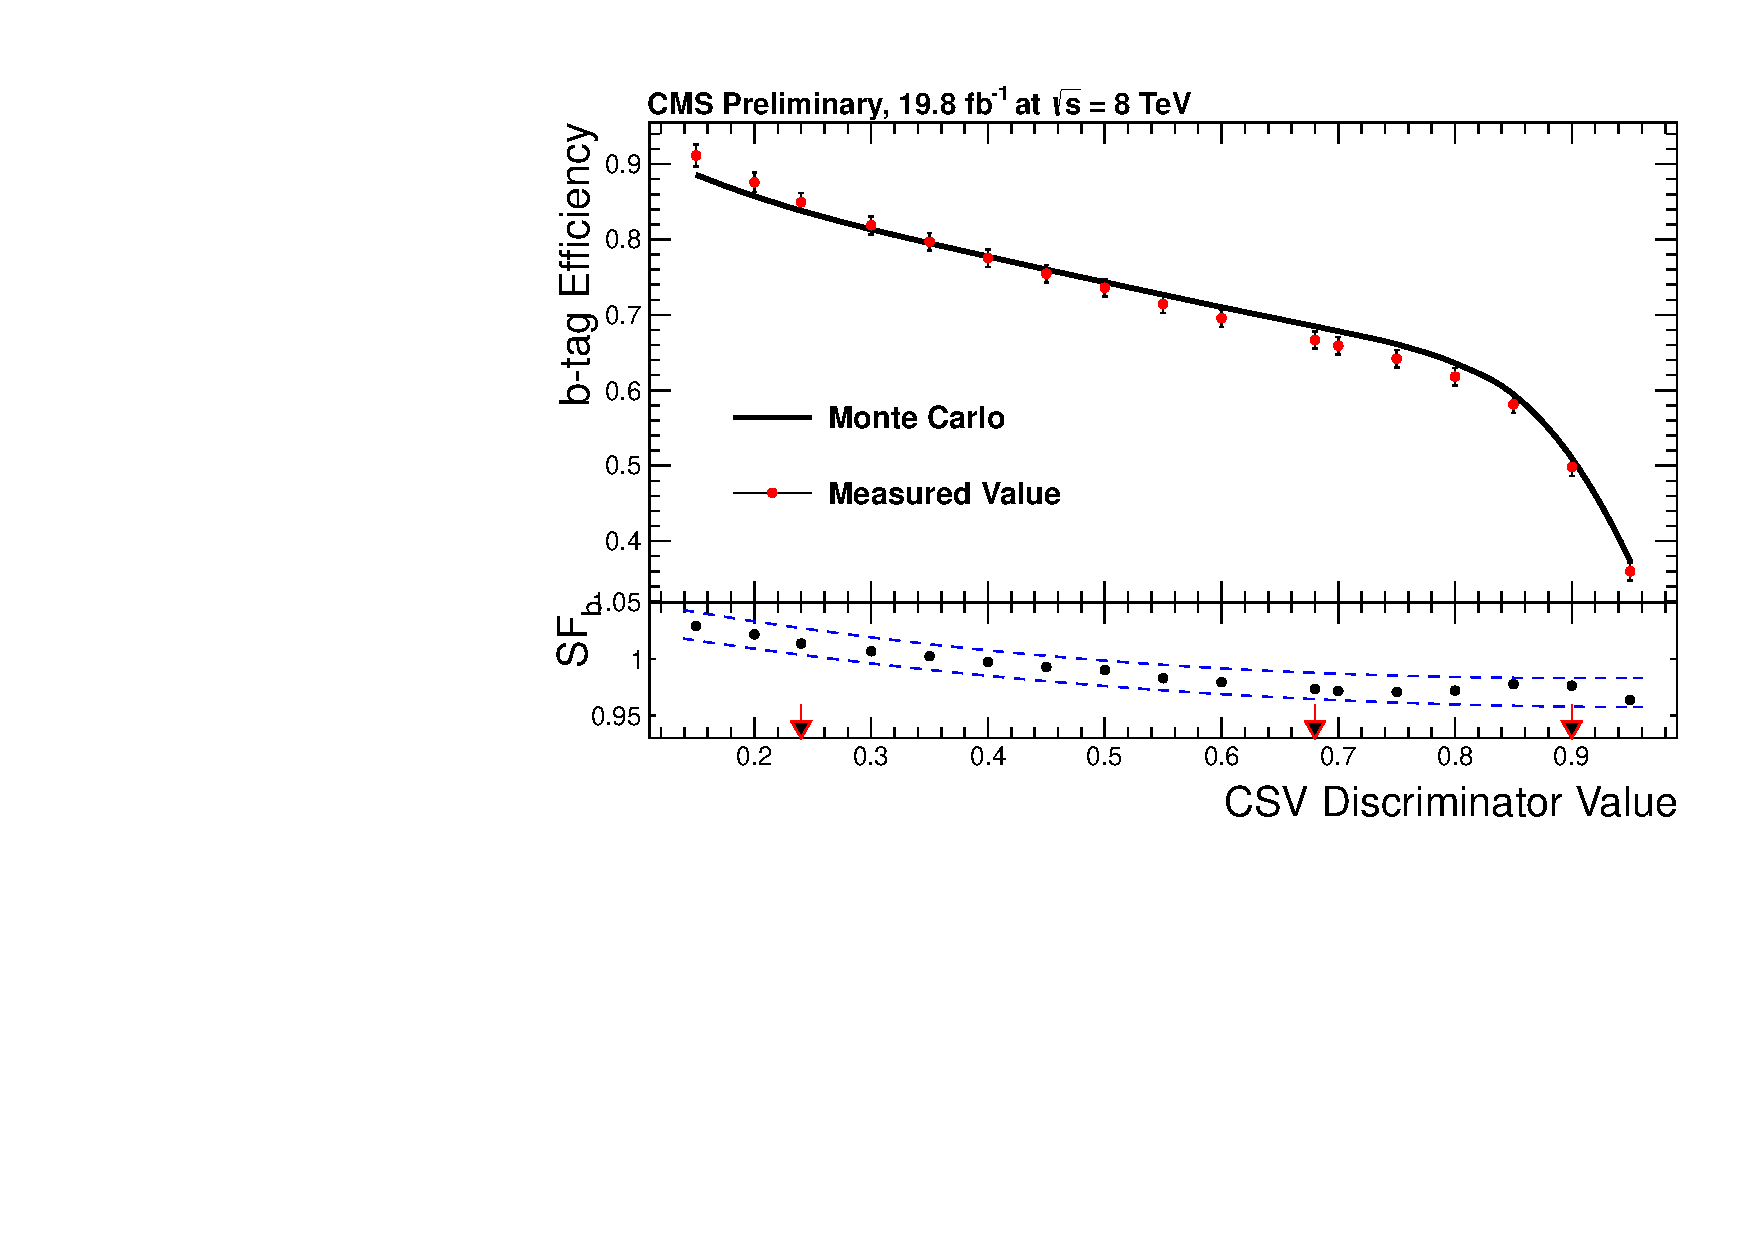
\includegraphics[width=0.6\textwidth]{04_event_reconstruction/plots/Figure_012-b.pdf}
  \caption{A b-jet tagging efficiency as a function of the discriminator threshold for the CSV algorithm. The three CSV working points are marked with the red arrows on the $x$-axis.
  The upper panel shows the efficiency measured in data and predicted from the simulation.
  The lower panel shows the ratio between data and simulation efficiencies, where the blue line represents the combined statistical and systematical uncertainty. The plot is taken from \cite{CMS-PAS-BTV-13-001}.}
  \label{fig:CSVeff}
\end{figure}

%%%%%%%%%%%%%%%%%%%%%%%%%%%%%%%%%%%%%%%%%%%%%%%
\subsection{Missing Transverse Energy}

There exists no transverse momentum component in the proton-proton collisions. Thus one expects to have a zero sum of the transverse momenta of the 
objects arising from the collisions out of the momentum conservation. This can be expressed the following way.

\begin{equation}\label{eq:EnBal}
 \sum_{detected\; objects} \vec{p}_{T} + \sum_{undetected\; objects} \vec{p}_{T} = 0.
\end{equation}

The sum of the undetected objects transverse momentum is the missing transverse energy $E_{T}^{miss}$.
It can be expressed from the eq. \ref{eq:EnBal} as an opposite vectorial sum of the transverse momenta over all reconstructed objects \cite{CMS-PAS-PFT-09-001}:

\begin{equation}
 \vec{E}^{miss}_{T} = - \sum_{detected\; objects} \vec{p}_{T}.
\end{equation}

% \begin{align}
%  \vec{E}_{T}^{miss} & = (E_{T_{x}}^{miss}, \, E_{T_{y}}^{miss}) = - \sum_{leptons} \vec{p}_{T}^{lepton} - \sum_{jets} \vec{p}_{T}^{jet}, \\
%  E_{T}^{miss} & = \sqrt{E_{T_{x}}^{miss^{2}} + E_{T_{y}}^{miss^{2}}}.
% \end{align}

Missing transverse energy reconstruction is sensitive to the pile up objects. To correct for the 
pile up effects the Multivariate Analysis (MVA) was performed \cite{CMS-PAS-JME-12-002}.
% The MVA is trained on the $Z \to e^{+}e^{-} / \mu^{+}\mu^{-}$ samples and attempts to distinguish between the events emerging from the hard interaction point and
% pile up vertecies. The improvement in resolution which the exploiting of the MVA for pile up rejection gives is $\sim 6\%$. However, the differences between data
% and simulation are getting larger. To compensate for these discrepancies the \textit{recoil corrections} are applied \cite{CMS-PAS-JME-12-002}. 

% A recoil $\vec{u}$ is calculated using the well reconstructed $Z \to e^{+}e^{-} / \mu^{+}\mu^{-}$ samples and is defined as shown in the eq. \ref{eq:recoil}:
% 
% \begin{equation}\label{eq:recoil}
%  \vec{u} = - \vec{p}_{T}(Z) - \vec{E}_{T}^{miss}
% \end{equation}
% 
% The parallel ($u_{||}$) and perpendicular ($u_{\perp}$) components with respect to the $Z$ direction are simultaneously fitted in data and simulation for each bin
% of the jet multiplicity and $p_{T}(Z)$. The areas of the fit curves $f$ in data and MC simulations are required to be equal:
% 
% \begin{equation}
%  \int_{-\infty}^{u_{corr}} f_{data}\; du = \int_{-\infty}^{u_{uncorr}} f_{sim.}\; du.
% \end{equation}
% 
% The corrected recoil value $u_{corr}$ is used to reestimate the missing transverse energy as $\vec{E}_{T}^{miss} = | \vec{p}_{T}(Z) - \vec{u}_{corr} |$.

%%%%%%%%%%%%%%%%%%%%%%%%%%%%%%%%%%%%%%%%%%%%%%%
%%%%%%%%%%%%%%%%%%%%%%%%%%%%%%%%%%%%%%%%%%%%%%%
%%%%%%%%%%%%%%%%%%%%%%%%%%%%%%%%%%%%%%%%%%%%%%%
\section{Event Selection and Correction}

The reconstructed objects in each event (which corresponds to one bunch crossing) have to fulfill certain criteria to be accepted for this analysis. These 
criteria are chosen taken to account the physical result this analysis is aiming for and the technical features of the CMS detector parts.

The incomplete correspondence of the simulation model to the experimental results has to be additionally corrected. The differences in the efficiencies 
of certain procedures in data and simulation are corrected by applying the \textit{Scale Factors}, $SF = \frac{\epsilon_{data}}{\epsilon_{MC}}$, 
on the MC distributions. Here $\epsilon_{data}$ is the efficiency determined in the experimental data and $\epsilon_{MC}$ is the efficiency from
simulation. 
%The overall differences of the experimental data and MC distributions is corrected via reweighing the simulation rates towards the experimental once.

All the selection requirements are summarized as follows:

\begin{itemize}
 \item [--] \textbf{Trigger selection}: The events have to be accepted by the HLT (see section \ref{sec:trig}) dilepton triggers, which require the presents of two leptons, electrons or muons, with
 minimum transverse momentum of 17 GeV and 8 GeV.
 
 The Scale Factors connected to the trigger selection were applied on the MC double-differentially in bins of two leptons rapidities. 
 %%%%% 
%  \item [--] \textbf{Beam scrapping}: Accept only events with maximum 10 reconstructed tracks, or more then 10 in case at least quarter of them has high quality of reconstruction.
 %%%%%
%  \item [--] \textbf{Calorimeter noise removal}: Event with anomalous calorimeter noise are removed.
 %%%%%
 \item [--] \textbf{Vertex requirement}: Only the hardest vertex (with the highest sum of the $p_{T}^{2}$ of the assigned tracks) is taken for the analysis. 
 \\
 An additional weight correction depending on a vertex multiplicity is applied on the MC. 
 The distributions presented in the figure \ref{fig:PUweight} show how the agreement
 between the experimental and simulated data improves after this reweighting is implemented.
 
 \begin{figure}[h]
 \centering
 \begin{subfigure}
   \centering
   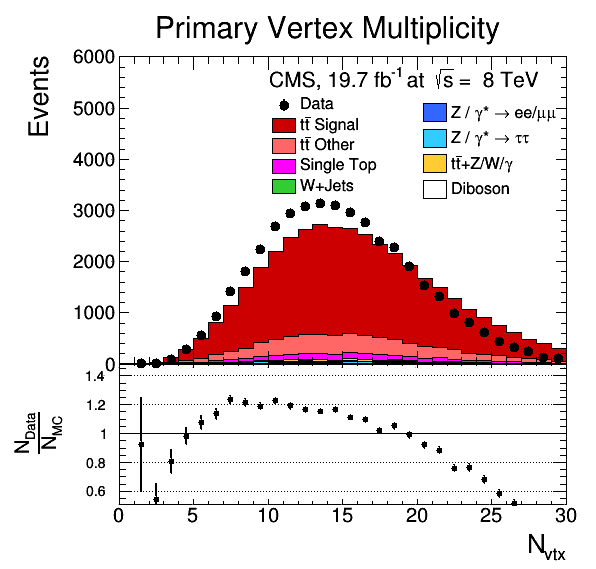
\includegraphics[width=0.49\textwidth]{04_event_reconstruction/plots/vertex_mult_noPUw.png}
 \end{subfigure}
 \begin{subfigure}
   \centering
   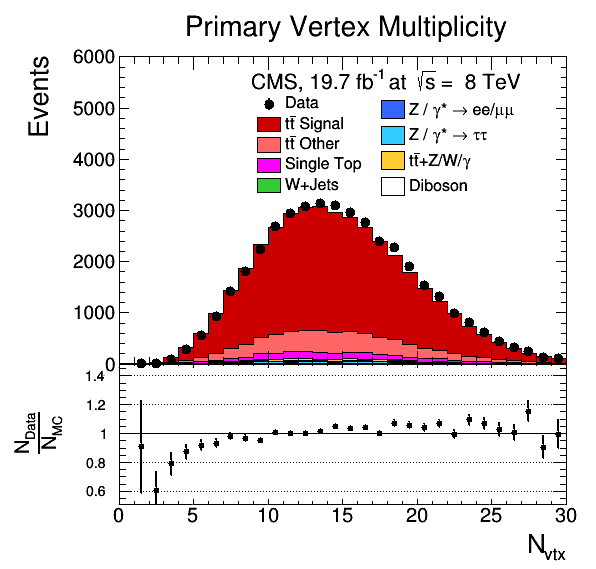
\includegraphics[width=0.49\textwidth]{04_event_reconstruction/plots/vertex_mult_PUw.png}
 \end{subfigure}
 \caption{The vertex multiplicity control distribution before (left) and after (right) the vertex correction reweighing after the whole selection.
 Black dots represent the experimental data and the colorful histograms are the MC simulation divided into signal and backgrounds contributions.
 The bottom plots represent the ratio between experimental and simulated data rates.}
 \label{fig:PUweight}
 \end{figure}
 
 %%%%%
 \item [--] \textbf{Lepton selection}: An event has to contain at least two opposite signed leptons (electron-muon pair) with $p_{T} > 20 \textrm{GeV}$ and $|\eta| < 2.4$.
 %%%%%
 \item [--] \textbf{Lepton isolation}: All the leptons in the event have to be isolated with $I_{rel}\leq 0.15$ in a cone of $\Delta R = 0.3$, where
 $I_{rel}$ is the relative isolation defined as:
  \begin{equation}\label{eq:Iso}
   I_{rel} = \frac{\sum E_{Tracker} + \sum E_{ECAL} + \sum E_{HCAL}}{p_{T}(l)}
  \end{equation}
 for a selected $\Delta R$ cone around the lepton track.
 
 As it is shown in the figure \ref{fig:PFIso}, the lepton isolation requirement cuts on the events which dominated by the QCD background and have a bad 
 agreement between experimental and simulated data and thus are cut away by the lepton isolation requirement.

 \begin{figure}[h]
 \centering
 \begin{subfigure}
   \centering
   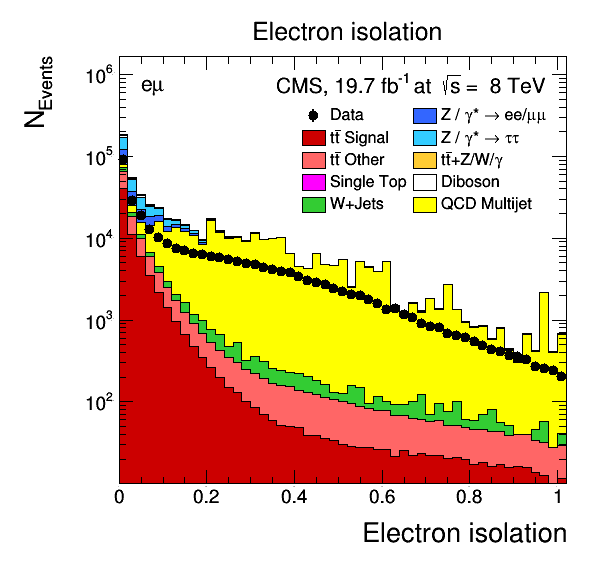
\includegraphics[width=0.49\textwidth]{04_event_reconstruction/plots/PF_e_Iso.png}
 \end{subfigure}
 \begin{subfigure}
   \centering
   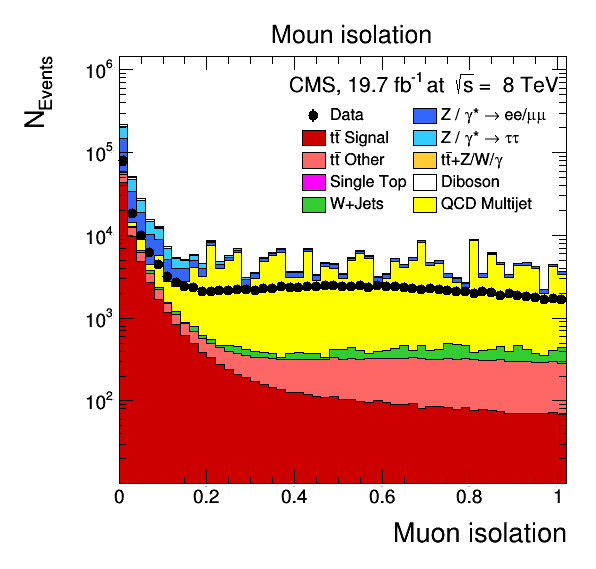
\includegraphics[width=0.49\textwidth]{04_event_reconstruction/plots/PF_mu_Iso.png}
 \end{subfigure}
 \caption{The electron (left) and muon (right) relative isolation $I_{rel}$ (\ref{eq:Iso}) control distributions displaying the experimental data points
 and simulated distributions of signal and different background after the trigger selection.}
 \label{fig:PFIso}
 \end{figure}
 %%%%%
 \item [--] \textbf{Lepton pair selection}: The mass of the system of two leading $p_{T}$ leptons has to be less then 20 GeV, otherwise the event is rejected. 
 %%%%%
 \item [--] \textbf{Jet selection}: The events which contain at least two jets with $p_{T} > 30$ GeV and $|\eta| \leq 2.4$ are accepted. The figure \ref{fig:jetMultiSel} shows 
 the jet multiplicity in the events, presenting that the events with less than two jets contain a significant fraction of the Drell-Yan background. 
 
 \begin{figure}[h]
  \centering
  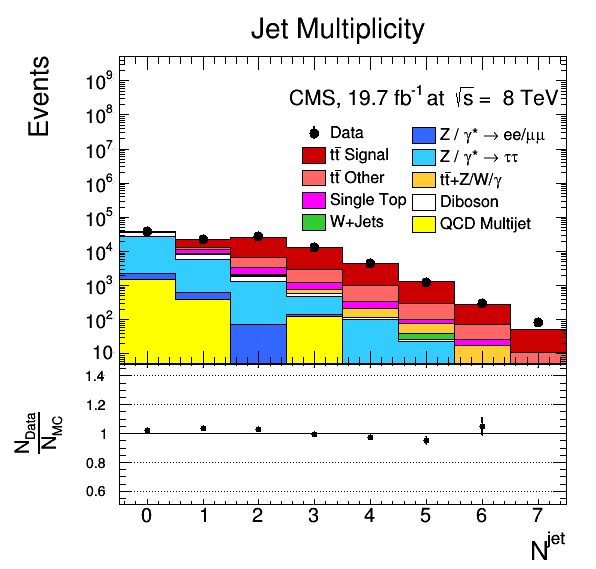
\includegraphics[width=0.6\textwidth]{04_event_reconstruction/plots/JetMulti.png}
  \caption{The control distribution of the jet multiplicity in the events after the trigger and lepton selection. The experimental data points
  and simulated distributions of signal and different background are plotted.}
  \label{fig:jetMultiSel}
 \end{figure}
 
 In the figure \ref{fig:mllJetSel} the dilepton mass before and after jet selection is shown, demonstrating a sizable background (especially Drell-Yan) fraction suppression power
 of the cuts implemented in this selection step.
 
 \begin{figure}[h]
 \centering
 \begin{subfigure}
   \centering
   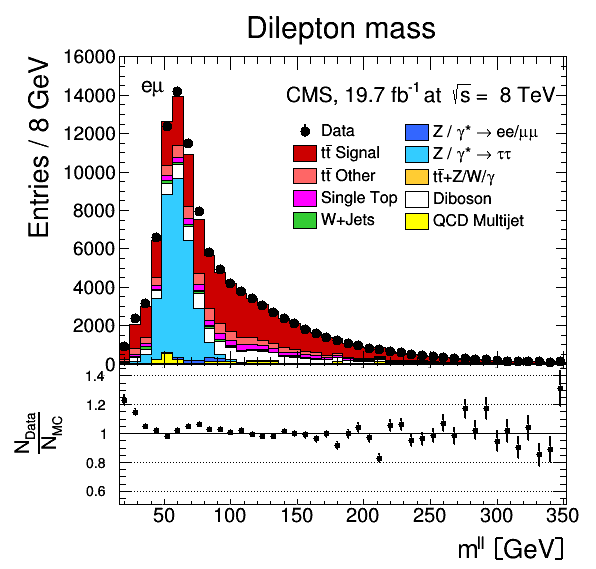
\includegraphics[width=0.49\textwidth]{04_event_reconstruction/plots/mll_step4.png}
 \end{subfigure}
 \begin{subfigure}
   \centering
   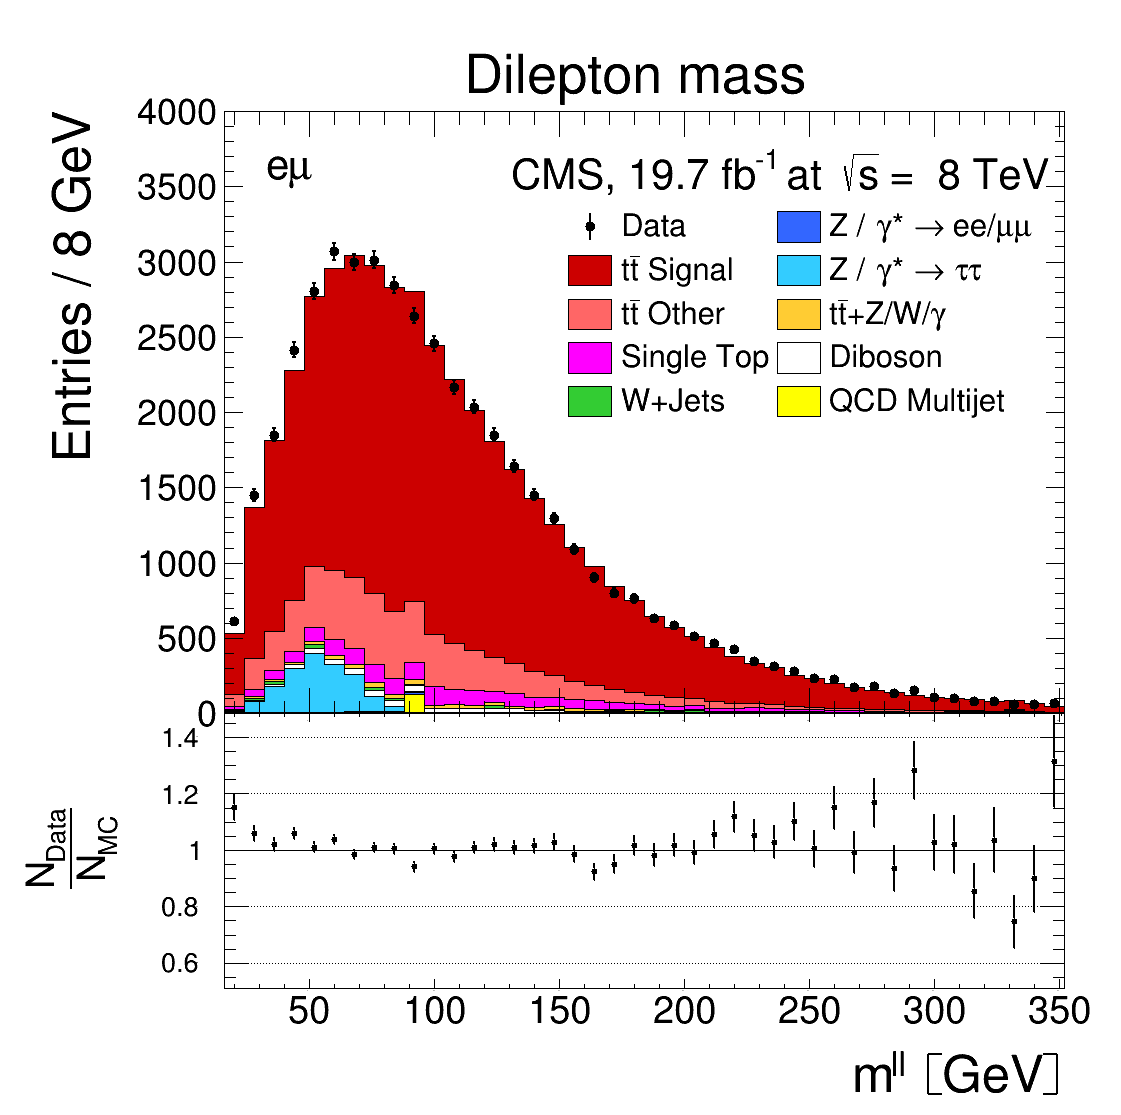
\includegraphics[width=0.49\textwidth]{04_event_reconstruction/plots/mll_step5.png}
 \end{subfigure}
 \caption{The control distribution of the dilepton mass in the events after the trigger and lepton selection (left) and after trigger, lepton and jet selection (right). 
 The experimental data points and simulated distributions of signal and different background are plotted.}
 \label{fig:mllJetSel}
 \end{figure}
 %
 \item [--] \textbf{$b$-jets selection}: An event has to contain at least one jet, tagged as originating from the $b$-quark with the help of CSVL. The multiplicity of the $b$-tagged
 jets is presented in the figure \ref{fig:bjetMultiSel} which shows that cutting out the events with no $b$-tagged jets should remove a sizable background fraction. Indeed, the figure \ref{fig:mllbJetSel} presenting
 the dilepton mall before and after the $b$-jets selection shows this background reduction.
 
 \begin{figure}[h]
  \centering
  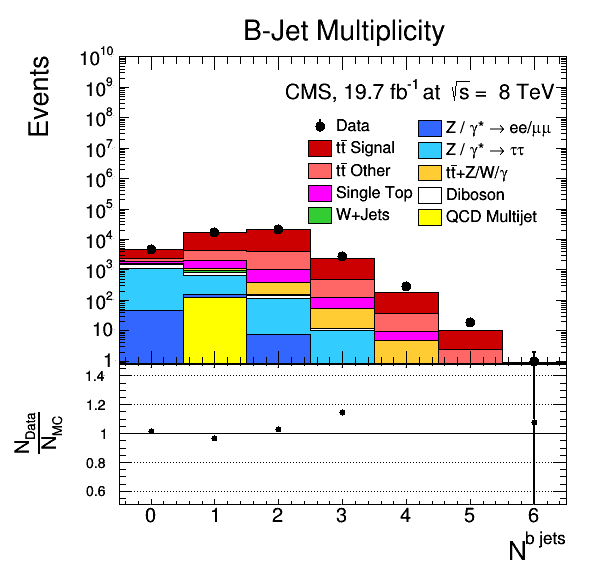
\includegraphics[width=0.6\textwidth]{04_event_reconstruction/plots/bJetMulti.png}
  \caption{The control distribution of the $b$-jet multiplicity in the events after the trigger, lepton and jet selection. The experimental data points
  and simulated distributions of signal and different background are plotted.}
  \label{fig:bjetMultiSel}
  \end{figure}
  
 \begin{figure}[h]
 \centering
 \begin{subfigure}
   \centering
   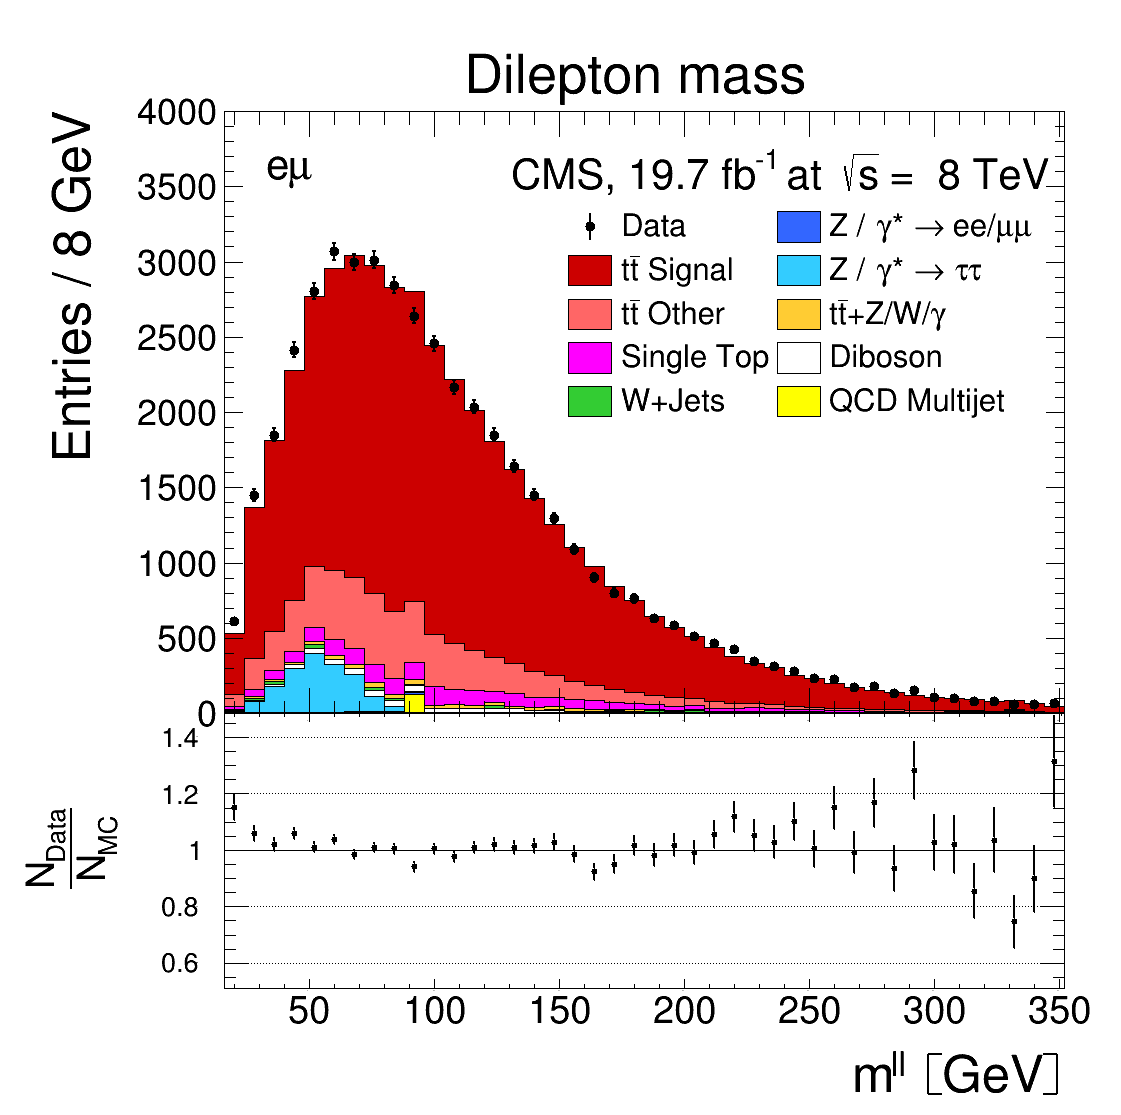
\includegraphics[width=0.49\textwidth]{04_event_reconstruction/plots/mll_step5.png}
 \end{subfigure}
 \begin{subfigure}
   \centering
   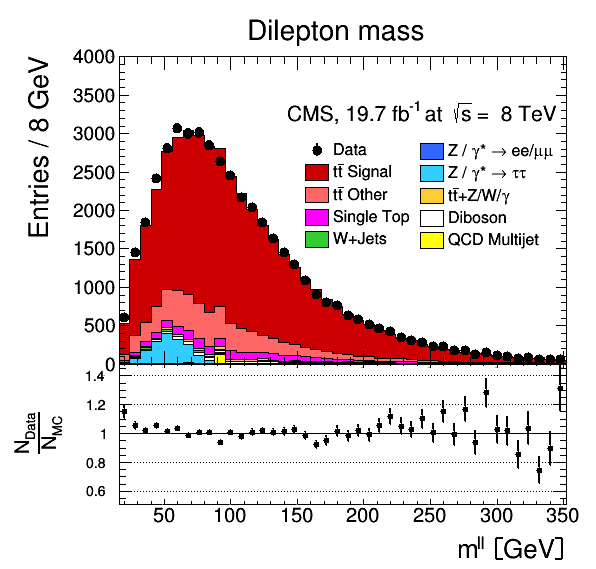
\includegraphics[width=0.49\textwidth]{04_event_reconstruction/plots/mll_step6.png}
 \end{subfigure}
 \caption{The control distribution of the dilepton mass in the events after the trigger, lepton and jet selection (left) and after trigger, lepton, jet and $b$-jet selection (right). 
 The experimental data points and simulated distributions of signal and different background are plotted.}
 \label{fig:mllbJetSel}
 \end{figure}
 %
 \end{itemize}

The set of selection criteria performs successfully decreasing the fraction of background events. The control distributions which show the data and MC simulation at one plot
contain all the background sources as a part of MC, thus providing a visualization of the outcoming results of the event selection process. 